
接下来,将要了解的下一组是性能分析工具。我们已经了解了性能分析器的使用,可以确定占用大量计算时间的函数。这正是其用途所在,它可以用来查找“热点”函数和代码片段,也就是程序花费最多时间的代码段。

有许多不同的商业和开源分析工具可供使用。本节中,我们将研究两个在Linux系统上主流的性能分析器。这里不是训练针对某个特定工具的专家,而仅是了解选择使用的性能分析器可以提供什么,以及如何对其结果进行解析。

首先,有几种不同类型的性能分析器:

\begin{itemize}
\item 一些分析器在解释器或虚拟机下执行,并观察各个代码段所花费的时间。这些分析器的主要缺点是,程序运行的速度比直接编译到机器指令的代码慢,至少对于像C++这样的编译语言来说,并且通常不会在虚拟机下运行的。

\item 还有一些分析器,要求在编译或链接期间用特殊的指令插入代码中。这些指令为分析器提供了相应的信息,例如:当函数被调用或循环开始和结束时,可以告知数据收集引擎。这些分析器比前一种类型的分析器快,但仍然比本机执行慢。并且,需要对代码进行特殊编译,并依赖于某种假设:插装的代码与原始代码的性能差异不大(如果不是绝对的,至少是相对的)。

\item 大多数现代分析器使用现代CPU上的硬件计数器。这些是硬件寄存器,可以用来跟踪某些硬件事件。硬件事件就是执行指令。可以看到这对分析非常有效:处理器将做计数指令的工作,而不需要其他工具或任何开销。我们需要做的就是读取计数寄存器的值而已。

\end{itemize}

或者,用简单地计算指令要复杂一点的方法。我们需要知道在每个函数中,甚至在每一行代码执行所花费的时间。如果分析器在执行每个函数(或每个循环、每一行代码,等等)之前和之后读取指令计数,就可以做到这一点。这就是为什么有分析器使用多种计数方案:使用特定的指令标记感兴趣的代码段,但使用硬件性能计数器来进行实际测量。

有些分析器依赖于时间采样:其以一定的间隔中断程序,例如:每10毫秒中断一次,并记录性能计数器的值,以及程序的当前位置(即将执行的指令)。如果90\%的样本在调用\texttt{compare()}函数的过程中获得的,则可以假设程序花了90\%的时间进行字符串比较。这种方法的准确性取决于采样数和采样率。

对程序执行的采样越频繁,收集的数据就越多,但开销也会越大。某些情况下,在采样不太频繁的情况下,可以使用硬件分析器,这就对程序的运行时间没有任何影响。

\subsubsubsection{2.4.1\hspace{0.2cm}perf分析器}

本节中的第一个分析器工具是Linux性能分析器。这是Linux上最流行的分析器之一,大多数发行版都有安装了,其是基于硬件性能计数器和基于时间采样的分析器。

运行这个分析器最简单的方法是收集整个程序的计数器值,可以通过\texttt{perf stat}命令完成:

%\hspace*{\fill} \\ %插入空行
\begin{center}
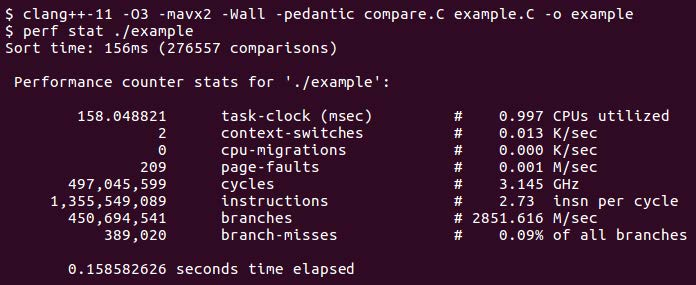
\includegraphics[width=0.9\textwidth]{content/1/chapter2/images/6.jpg}\\
图 2.6
\end{center}

从图2.6中可以看到,编译不需要任何特殊选项或工具。程序由分析器执行,\texttt{stat}选项告诉分析器显示在程序运行期间,硬件性能计数器中累积的计数值。本例中,程序运行了158毫秒(与程序本身打印的时间一致),并执行了13亿多条指令。还显示了其他几个计数器,如“页面错误”和“分支”。这些计数器是什么,还有哪些计数器?

事实证明,现代CPU可以收集不同类型事件的统计信息,但一次只能收集几种类型的事件。前面的例子中,报告了8个计数器,因此可以假设这个CPU有8个独立的计数器。以前,每个计数器都会分配到一个事件类型中。分析器本身可以列出所有已知的事件,并可以计数:

%\hspace*{\fill} \\ %插入空行
\begin{center}
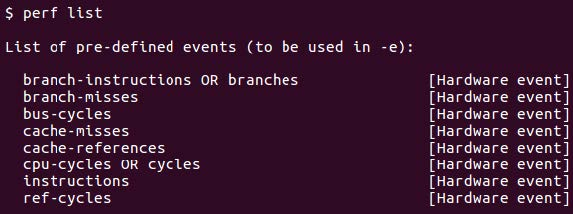
\includegraphics[width=0.9\textwidth]{content/1/chapter2/images/7.jpg}\\
图 2.7
\end{center}

图2.7中的列表是不完整的(打印输出会有很多行),可用的计数器因CPU而异(如果使用虚拟机,则在管理程序的类型和配置上有所不同)。图2.6中的结果只是默认配置的计数器收集的,我们还可以选择其他的计数器进行配置:

%\hspace*{\fill} \\ %插入空行
\begin{center}
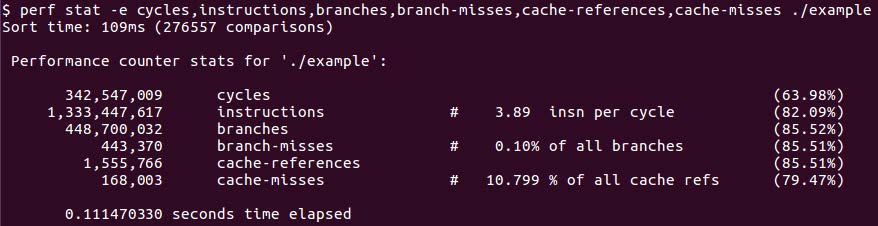
\includegraphics[width=0.9\textwidth]{content/1/chapter2/images/8.jpg}\\
图 2.8
\end{center}

图2.8中,我们可以测量CPU周期和指令,以及分支、分支缺失、缓存引用和缓存缺失。下一章将详细解释这些计数器和其相应的监视事件。

简单地说,周期时间是CPU频率的倒数,所以一个3GHz的CPU每秒可以运行30亿个周期。大多数CPU的频率是可变的,这使得测量变得更复杂了。因此,为了精确的分析和进行基准测试,建议禁用省电模式和其他会让CPU时钟变化的功能。指令计数器测量处理器执行指令的数量,CPU平均每周期可以执行四条指令。

“分支”是条件指令:每个带有条件的\texttt{if}语句和每个\texttt{for}循环都会生成多条这样的指令。分支缺失在下一章进行解释,现在从性能的角度来看,我们只能说这是一个性能开销大,而且不受欢迎的事件。

“缓存引用”计算CPU需要从内存中读取的次数。大多数时候是一段数据,比如:字符串中的一个字符。根据处理器和内存的状态,这个取回可以非常快,也可以非常慢。慢的话会认为是“缓存丢失”(“慢”是一个相对概念:相对于3ghz的处理器速度,1微秒是一个很长的时间)。内存层次结构将在后面的章节进行解释。而且,缓存丢失也是一个性能开销特别大的事件。

理解了CPU和内存的工作方式后,就能够使用这些度量来衡量程序的总体效率,并确定哪些因素限制了程序的性能。

到目前为止,我们只看到了整个项目的测量结果。图2.8中告诉我们哪些事件拖累了代码的性能,例如:如果我们现在接受“缓存丢失”对性能不利的观点,可以推断出这段代码的主要问题是低效的内存访问(十分之一的内存访问是缓慢的)。然而,这种类型的数据并没有告诉我们,代码具体是哪部分导致了较差的性能。为此,不仅需要在程序执行之前和之后收集数据,还需要在程序执行期间收集数据。让我们看看如何用\texttt{perf}来收集这些信息。

\subsubsubsection{2.4.2\hspace{0.2cm}使用perf进行详细分析}

\texttt{perf}分析器将硬件计数器与基于时间采样结合起来,记录正在运行的程序的性能情况。对于每个示例,记录程序计数器的位置(要执行的指令的地址)和需要监视的性能计数器。运行后,对数据进行分析,包含大多数的函数和代码行的执行时间。

分析器的数据收集运行并不比整体测量运行更困难。注意,在运行时,回收集指令地址,从而转换为原始源代码中的行号,程序必须使用调试信息进行编译。若已经习惯了“优化”和“非优化”这两种编译模式,这种编译器选项的组合可能会让您惊讶:调试和优化都启用。启用后者的原因是,我们需要配置将在生产环境中运行的相同代码;否则,数据没什么无意义。考虑到这一点,我们可以编译代码来分析,并使用\texttt{perf record}命令运行分析器:

%\hspace*{\fill} \\ %插入空行
\begin{center}
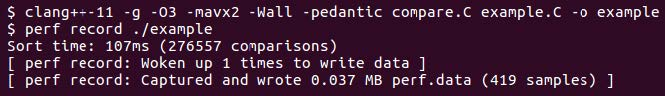
\includegraphics[width=0.9\textwidth]{content/1/chapter2/images/9.jpg}\\
图 2.9
\end{center}

与\texttt{perf stat}类似,可以指定计数器或一组计数器。但是这次,我们使用默认计数器。我们没有具体说明采样的频率,使用默认值。采样频率可以显示的进行指定,例如:\texttt{perf record -c 1000}即记录每秒1000个样本。

The program runs, produces its regular output, as well as the messages from the profiler. The last one tells us that the profiling samples have been captured in the file named perf.data (again, this is the default that can be changed). To visualize the data from this file, we need to use the profile analysis tool, which is also a part of the same perftools suite, specifically, the perf report command. Running this command will launch this screen:

%\hspace*{\fill} \\ %插入空行
\begin{center}
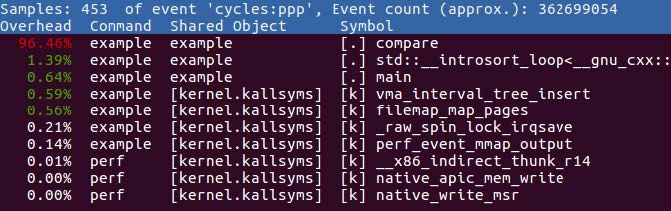
\includegraphics[width=0.9\textwidth]{content/1/chapter2/images/10.jpg}\\
图 2.10
\end{center}

This is the profiling summary, a breakdown of the execution time by function. From here, we can drill down into any function and see which lines contributed the most to the execution time:

%\hspace*{\fill} \\ %插入空行
\begin{center}
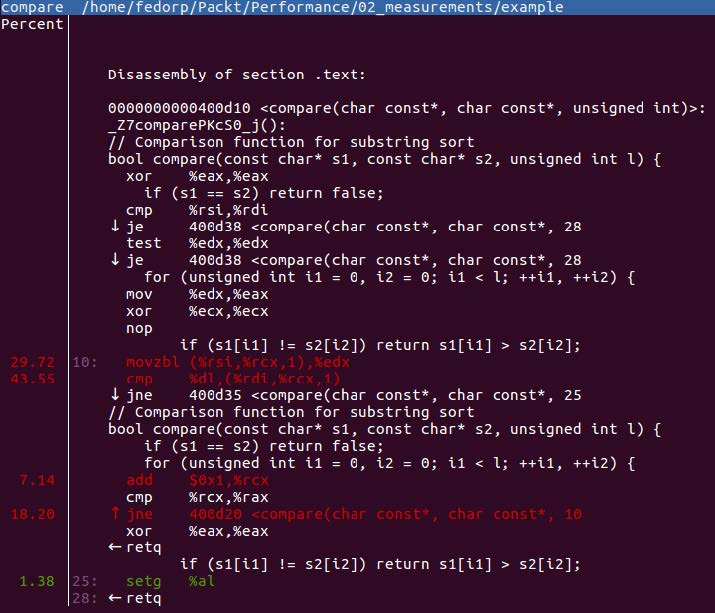
\includegraphics[width=0.9\textwidth]{content/1/chapter2/images/11.jpg}\\
图 2.11
\end{center}

The numbers on the left in Figure 2.11 are the percentages of the execution time spent at each line. So, what exactly does the "line" tell us? Figure 2.11 illustrates one of the more frequent difficulties in analyzing such profiles. It shows both the source code and the assembly instructions produced from it; the execution time counters are, naturally, associated with every hardware instruction (that is what the CPU executes, so that's the only thing it can count). The correspondence between the compiled code and the source is established by the profiler using the debugging information embedded by the compiler. Unfortunately, this correspondence is not exact, and the reason for this is optimization. The compiler performs a wide range of optimizations, all of which end up rearranging the code and changing the way the computations are done. You can see the results even in this very simple example: why does the source code line

\begin{lstlisting}[style=styleCXX]
if (s1 == s2) return false;
\end{lstlisting}

the instructions generated from this line are not all in the same place; the optimizer reordered them with the instructions originating from other lines. So the profiler shows this line near both machine instructions that were originally generated from it.

Even without looking at the assembler, we can see that the time is spent comparing the characters, as well as running the loop itself; these two source lines account for most of the time:

\begin{lstlisting}[style=styleCXX]
for (unsigned int i1 = 0, i2 = 0; i1 < l; ++i1, ++i2) {
	if (s1[i1] != s2[i2]) return s1[i1] > s2[i2];
\end{lstlisting}

To get the most out of the profile, it helps to understand at least the basics of the assembly language of the platform we're working on (X86 CPUs, in our case). The profiler also has some helpful tools that facilitate the analysis. For example, by placing the cursor on the jne (jump if not equal) instruction, we can see where the jump would take us, as well as the condition associated with the jump:

%\hspace*{\fill} \\ %插入空行
\begin{center}
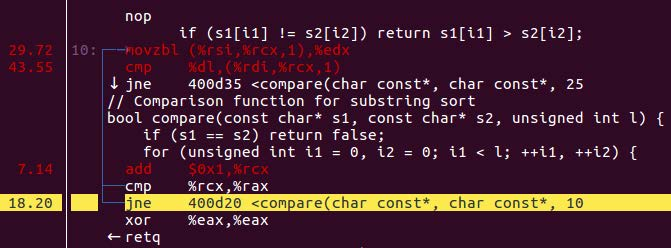
\includegraphics[width=0.9\textwidth]{content/1/chapter2/images/12.jpg}\\
图 2.12
\end{center}

This looks like a jump back to repeat the last few lines of code, so the cmp (compare) instruction above the jump must be the comparison of the loop, i1 < l. Together, the jump and the comparison account for 18\% of the execution time, so our earlier attention to the seemingly unnecessary comparison operation appears justified.

The perf profiler has many more options and capabilities for analyzing, filtering, and aggregating the results, all of which you can learn from its documentation. There are also several GUI frontends for this profiler. Next, we are going to take a quick look at another profiler, the one from Google Performance tools.

\subsubsubsection{2.4.3\hspace{0.2cm}The Google Performance profiler}

The Google CPU profiler also uses hardware performance counters. It also requires link-time instrumentation of the code (but no compile-time instrumentation). To prepare the code for profiling, you have to link it with the profiler library:

%\hspace*{\fill} \\ %插入空行
\begin{center}

\includegraphics[width=0.9\textwidth]{content/1/chapter2/images/13.jpg}\\
图 2.13
\end{center}

In Figure 2.13, the library is specified by the command-line option –lprofiler. Unlike perf, this profiler does not need any special tools to invoke the program; the necessary code is already linked into the executable. The instrumented executable does not automatically start profiling itself. We have to activate the profiling by setting the environment variable CPUPROFILE to the filename of the file where we want to store the results. Other options are also controlled through the environment variables instead of command-line options, for example, the variable CPUPROFILE\_FREQUENCY sets the number of samples per second:

%\hspace*{\fill} \\ %插入空行
\begin{center}
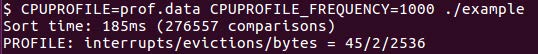
\includegraphics[width=0.9\textwidth]{content/1/chapter2/images/14.jpg}\\
图 2.14
\end{center}

Again, we see the output from the program itself and from the profiler, and we get the profile data file that we must analyze. The profiler has both the interactive and the batch mode; the interactive mode is a simple text user interface:

%\hspace*{\fill} \\ %插入空行
\begin{center}
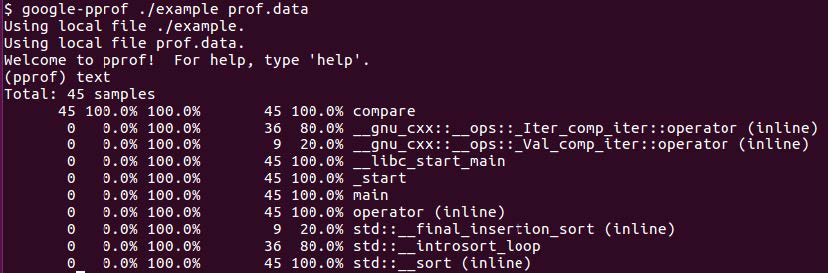
\includegraphics[width=0.9\textwidth]{content/1/chapter2/images/15.jpg}\\
图 2.15
\end{center}

Simply running google-pprof (often installed as just pprof) with the names of the executable and the profile as arguments brings up the command prompt. From here, we can, for example, get the summary of all functions annotated with percentages of the execution time. We can further analyze the program performance at the source code level:

%\hspace*{\fill} \\ %插入空行
\begin{center}
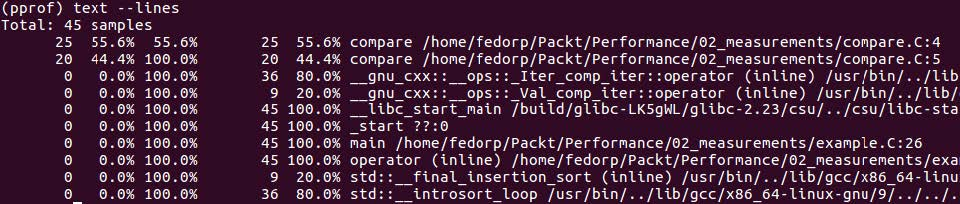
\includegraphics[width=0.9\textwidth]{content/1/chapter2/images/16.jpg}\\
图 2.16
\end{center}

As you can see, this profiler takes a slightly different approach and does not immediately dump us, neck-deep, into machine code (although annotated assembly can also be produced). This apparent simplicity is somewhat deceptive, though: the caveats we described earlier still apply, the optimizing compiler still does its transformations on the code.

Different profilers have somewhat different strengths and weaknesses, owing to the different approaches taken by their authors. Without turning this chapter into a profier manual, we will show in the rest of this section some of the more common problems you may encounter when collecting and analyzing the profile.

\subsubsubsection{2.4.4\hspace{0.2cm}Profiling with call graphs}

So far, our simple example has avoided one problem that, in reality, happens in every program. When we discovered that the comparison function is responsible for the majority of the execution time, we immediately knew which part of the program is responsible: there was only one line that calls this function.

Most real-life programs are not so simple: after all, one of the main reasons we write functions is to facilitate code reuse. It stands to reason that many functions will be called from multiple locations, some many times and others just a few times, often with very different parameters. Simply knowing which function takes a lot of time is not enough: we also need to know in which context it happens (after all, the most effective optimization may be to call the expensive function less often).

What we need is a profile that does not just tell us how much time is spent in each function and on each line of code, but also how much time is spent in each call chain. These profilers usually present this information using the call graphs: graphs where callers and callees are nodes and calls are edges.

First, we have to modify our example so we can call some function from more than one location. Let us start by making two sort calls:

\hspace*{\fill} \\ %插入空行
\noindent
\textbf{05\_compare\_timer.C}
\begin{lstlisting}[style=styleCXX]
std::sort(vs.begin(), vs.end(),
  [&](const char* a, const char* b) {
	++count; return compare1(a, b, L); });
std::sort(vs.begin(), vs.end(),
  [&](const char* a, const char* b) {
	++count; return compare2(a, b, L); });
\end{lstlisting}

The calls differ only in the comparison functions; in our case, the first comparison function is the same as before, and the second one produces the opposite order. The two functions have the same loop over substring characters as our old comparison function:

\hspace*{\fill} \\ %插入空行
\noindent
\textbf{05\_compare\_timer.C}
\begin{lstlisting}[style=styleCXX]
bool compare1(const char* s1, const char* s2, unsigned int l) {
	if (s1 == s2) return false;
	for (unsigned int i1 = 0, i2 = 0; i1 < l; ++i1, ++i2) {
		int res = compare(s1[i1], s2[i2]);
		if (res != 0) return res > 0;
	}
	return false;
}
bool compare2(const char* s1, const char* s2, unsigned int l) {
	if (s1 == s2) return false;
	for (unsigned int i1 = 0, i2 = 0; i1 < l; ++i1, ++i2) {
		int res = compare(s1[i1], s2[i2]);
		if (res != 0) return res < 0;
	}
	return false;
}
\end{lstlisting}

Both functions use the same common function to compare each character:

\begin{lstlisting}[style=styleCXX]
int compare(char c1, char c2) {
	if (c1 > c2) return 1;
	if (c1 < c2) return -1;
	return 0;
}
\end{lstlisting}

This isn't, of course, how you would do it in a real program: if you really wanted to avoid the code duplication caused by repeating the loop, you would write a single function parametrized by the character comparison operator. However, we do not want to deviate too far from the example we started with, and we want to keep the code simple so we can explain the results one complication at a time.

Now we are ready to produce a call graph that will show us how the cost of the character comparison is split between the two calls to sort. Both profilers we have used can produce call graphs; in this section, we will use the Google profiler. For this profiler, data collection already included the call chain information; we just haven't tried to visualize it so far.

We compile the code and run the profiler exactly as we did it earlier (for simplicity, we put each function in its own source file):

%\hspace*{\fill} \\ %插入空行
\begin{center}
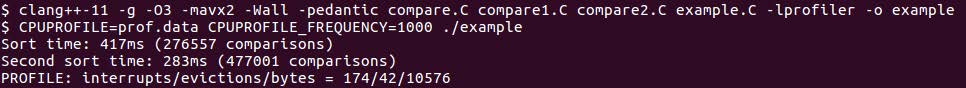
\includegraphics[width=0.9\textwidth]{content/1/chapter2/images/17.jpg}\\
图 2.17
\end{center}

The profiler can show the call graph in several different formats (Postscript, GIF, PDF, and so on). For example, to generate the PDF output, we would run this command:

\begin{tcblisting}{commandshell={}}
google-pprof --pdf ./example prof.data > prof.pdf
\end{tcblisting}

The information we're interested in right now is at the bottom of the call graph: 

%\hspace*{\fill} \\ %插入空行
\begin{center}
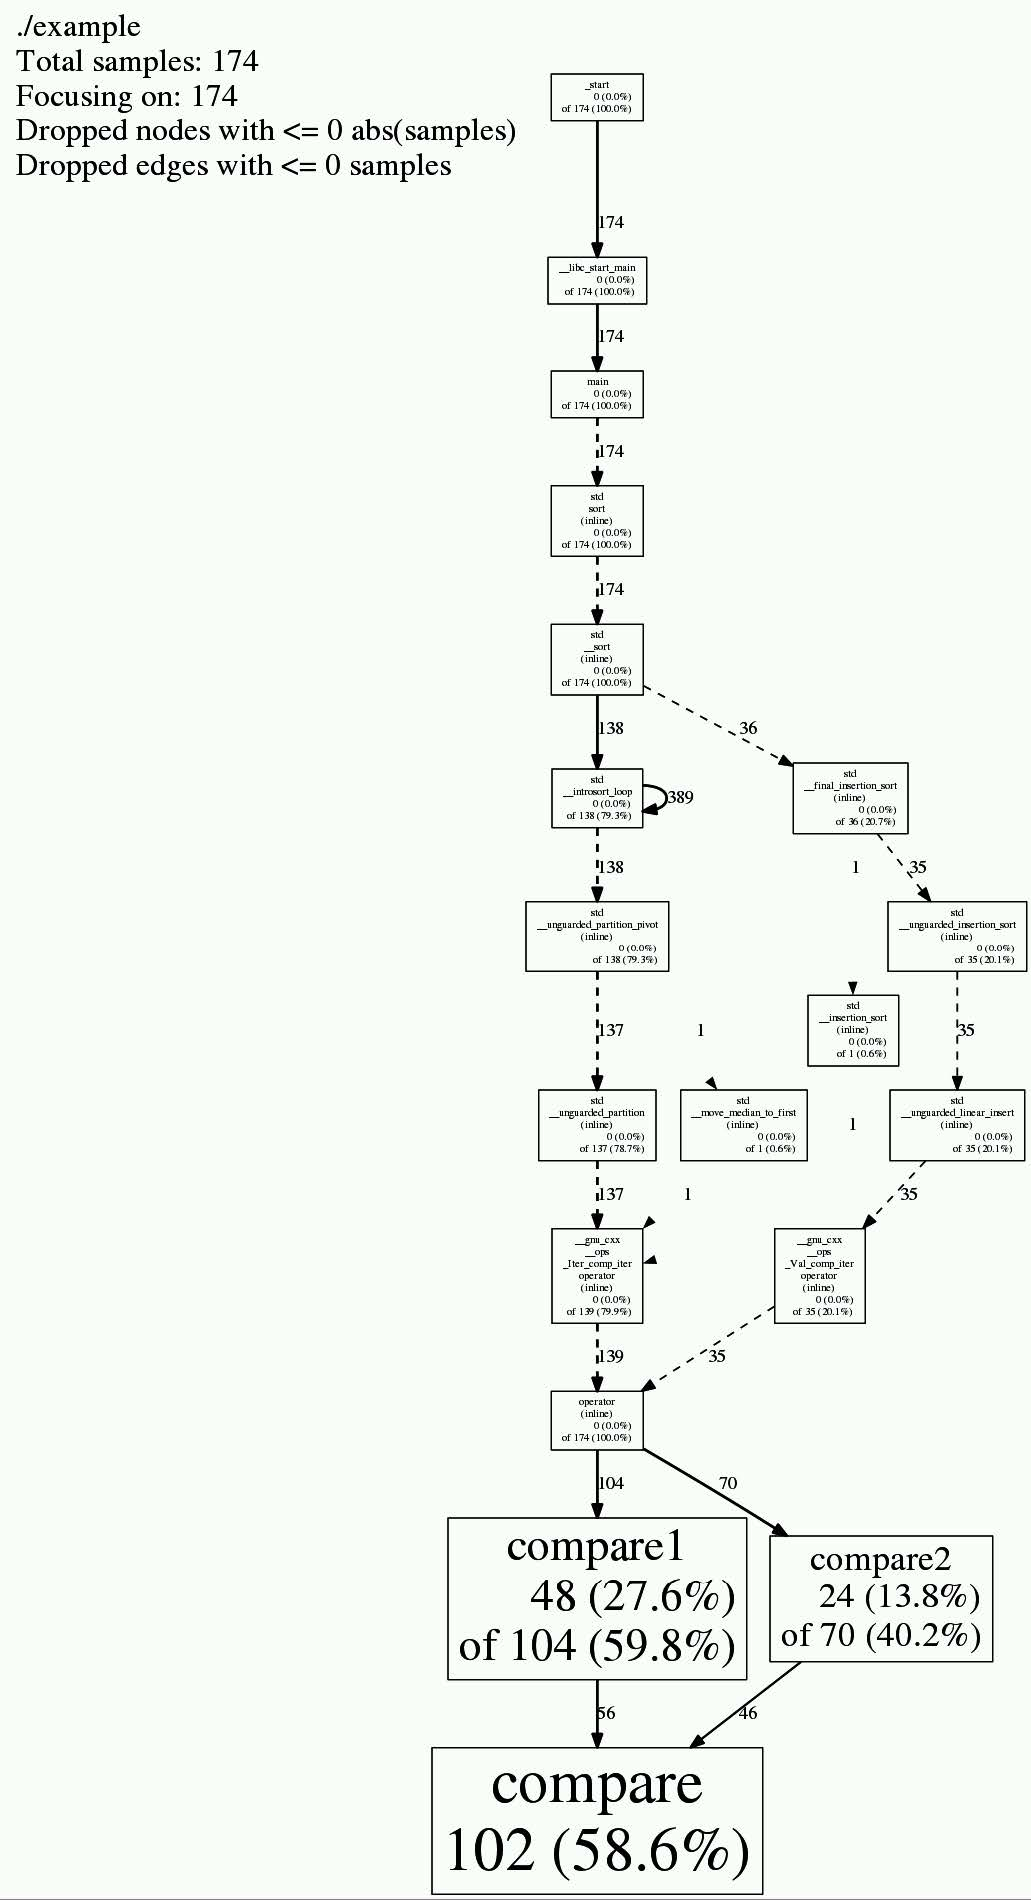
\includegraphics[width=0.9\textwidth]{content/1/chapter2/images/18.jpg}\\
图 2.18
\end{center}

As you can see in Figure 2.18, the compare() function, which accounts for 58.6\% of the total execution time, has two callers. Of the two, the compare1() function makes slightly more calls than the compare2() function; the former accounts for 27.6\% of the execution time (or 59.8\% if you include the time spent in its share of calls to compare()) and the latter is responsible for 13.8\% of the time by itself, or 40.2\% in total.

The basic call graphs are often enough to identify the problem call chains and select areas of the program for further exploration. Profiling tools also have more advanced reporting capabilities, such as the filtering of function names, aggregation of results, and so on. Mastering the features of your chosen tool can be the difference between knowledge and guesswork: interpreting performance profiles can be tricky and frustrating, and there are many reasons for it: some arise from tool limitations, but others are more fundamental. In the next section, we will talk about one of the latter reasons: for the measurements to be relevant, they must be done on fully optimized code.

\subsubsubsection{2.4.5\hspace{0.2cm}Optimization and inlining}

We have already seen how compiler optimization muddies the waters when it comes to interpreting performance profiles: all profiling is done, at the end of the day, on the compiled machine code, while we see the program in its source form. The relation between these two forms is obscured by compiler optimizations. One of the most aggressive optimizations, in terms of rearranging the source code, is compile-time inlining of function calls.

The inlining requires that the source of the function be visible at the call site, so, in order to show you how this looks, we have to combine the entire source code in one file:+

\hspace*{\fill} \\ %插入空行
\noindent
\textbf{02\_substring\_sort.C}
\begin{lstlisting}[style=styleCXX]
bool compare(const char* s1, const char* s2, unsigned int l) {
	if (s1 == s2) return false;
	for (unsigned int i1 = 0, i2 = 0; i1 < l; ++i1, ++i2) {
		if (s1[i1] != s2[i2]) return s1[i1] > s2[i2];
	}
	return false;
}
int main() {
	…
	size_t count = 0;
	std::sort(vs.begin(), vs.end(),
	  [&](const char* a, const char* b) {
		++count; return compare(a, b, L); });
}
\end{lstlisting}

Now the compiler can, and probably will, generate the machine code for the comparison right where it is used by the sort, instead of calling the external function. Such inlining is a potent optimization tool; it happens quite often and not just with functions from the same file. Much more often, inlining affects header-only functions (functions whose entire implementation is in the header file). For example, in the preceding code, the call to std::sort, which looks like a function call, is almost certainly inlined because std::sort is a template function: its entire body is in the header files.

Let us see how the profiler tools we used earlier deal with the inlined code. Running the Google profiler for annotated source lines produces this report:

%\hspace*{\fill} \\ %插入空行
\begin{center}
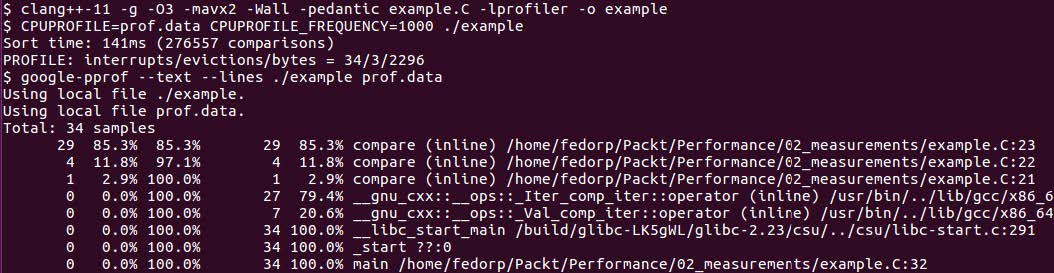
\includegraphics[width=0.9\textwidth]{content/1/chapter2/images/19.jpg}\\
图 2.19
\end{center}

As you can see, the profiler knows that the compare() function was inlined but still shows its original name. The lines in the source code correspond to the location where the code for the function is written, not where it is called, for example, line 23 is this line:

\begin{lstlisting}[style=styleCXX]
if (s1[i1] != s2[i2]) return s1[i1] > s2[i2];
\end{lstlisting}

The perf profiler, on the other hand, does not show inline functions as easily:

%\hspace*{\fill} \\ %插入空行
\begin{center}
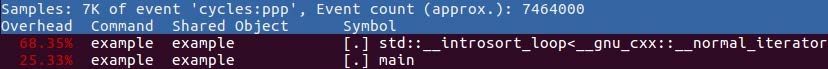
\includegraphics[width=0.9\textwidth]{content/1/chapter2/images/20.jpg}\\
图 2.20
\end{center}

Here we can see that the time appears to be spent in the sort code and the main program itself. Examining the annotated source, however, shows us that the code that was generated from the compare() function's source is still responsible for the absolute majority of the execution time:

%\hspace*{\fill} \\ %插入空行
\begin{center}
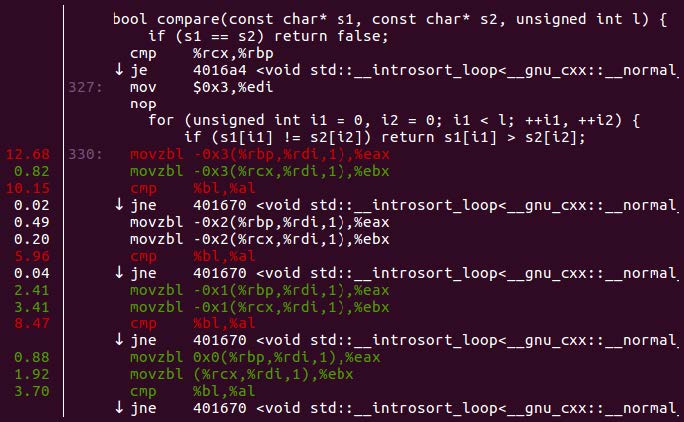
\includegraphics[width=0.9\textwidth]{content/1/chapter2/images/21.jpg}\\
图 2.21
\end{center}

There is, unfortunately, no easy way to undo the effects of the optimizations on the performance profiles. Inlining, code reordering, and other transformations turn detailed performance analysis into a skill that develops with practice. Perforce, some practical suggestions for the effective use of profiling are now in order.

\subsubsubsection{2.4.6\hspace{0.2cm}Practical profiling}

It may be tempting to think of profiling as the ultimate solution to all your performance measurement needs: run the whole program under a profiler, collect all the data, and get the complete analysis of everything that is going on in the code. Unfortunately, it rarely works out this way. Sometimes, the tool limitations get in the way. Often, the complexity of the information contained in the large amounts of data is simply too overwhelming. How, then, should you use profiling effectively?

The recommended approach is to collect high-level information first, then refine it. A coarse profile that breaks down the execution time between large modules may be a good place to start. On the other hand, you may have that information already if the modules are instrumented for benchmarking and have timers bracketing all major execution steps. If you don't have such instrumentation, the initial profile offers good suggestions for what these steps are, so consider adding the benchmarking instrumentation now, so you have them next time: you don't really expect to solve all your performance problems once and for all, do you?

With the benchmarking results and the coarse profile, you will likely encounter one of several scenarios. If you are very lucky, the profile will point to some low-hanging fruit, like a function that takes 99\% of the time doing a sort of a list. Yes, it happens: nobody expected the list to be longer than ten elements when the code was first written, and so it was for a while, and then everyone forgot about that code until it showed up as the long pole on the profile.

More likely, the profile will lead you to some large functions or modules. Now you have to iterate, create tests that focus on the interesting parts of the program, and profile a smaller portion of the code in more detail. Some amount of benchmarking data can also be very helpful in interpreting the profiles: while the profile will tell you how much time was spent in a given function or a loop, it won't count loop iterations or trace through if-else conditions. Note that most profilers can count function calls, so a good modular code is easier to profile than a huge monolithic mess.

As you collect and refine the profiles, the data will guide your attention toward the performance-critical areas of the code. It is also the point where you can fall into a common error: as you are focused on the code that is too slow, you may jump to optimizing it without considering the bigger picture. For example, the profile shows that a particular loop spends most time in memory allocation. Before you decide that you need a more efficient memory allocator, consider whether you actually need to allocate and deallocate memory on every iteration of the loop. The best way to make slow code faster is often to call it less often. This may require a different algorithm or just a more efficient implementation.

Just as often, you will discover that there is a computation you must do, it is the performance-critical part of the code, and the only way to speed up the program is to make this code faster. Now you have to try different ideas for optimizing it and see what works best. You can do it live in the program itself, but often this is a wasteful approach that significantly reduces your productivity. Ideally, you want to quickly experiment with different implementations or even different algorithms for a particular problem. It is here that you can take advantage of the third method for collecting performance data, microbenchmarking.













